\documentclass[../../../../main.tex]{subfiles}
\begin{document}

\begin{flushright}
\footnotesize\textit{【自動文字起こし・要確認】}
\end{flushright}

[解] 題意より、容器の $0 \le z \le f(t)$ の部分の体積が、回転体の先端からの長さ $t + f(t)$ までの部分の体積に等しいので、
\[ \pi R^2 \cdot f(t) = \int_0^{f(t)+t} \pi r(z)^2 dz \]
$f(t) = e^t - t - 1$ を代入、微分して
\[ R^2(e^t - t - 1) = \int_0^{e^t - 1} r(z)^2 dz \cdots \text{①} \]
①の両辺を $t$ で微分して、
\[ R^2(e^t - 1) = e^t r(e^t - 1)^2 \]
$r(z)$の定義域は $0 \le z$ だから、
$z = e^t - 1$ とおいて、
\[ R^2 z = (z+1) r(z)^2 \]
\[ r(z) = \pm R \sqrt{\frac{z}{z+1}} \]
このうち、$0 \le r(z) < R$ をみたす複号正を採用して
\[ r(z) = R \sqrt{\frac{z}{z+1}} \quad (r(0)=0 \text{をみたす}) \]

\begin{center}
\begin{tikzpicture}
% Left diagram
\draw[->] (-1.5, 0) -- (1.5, 0) node[right] {$x$};
\draw[->] (0, -2) -- (0, 2) node[above] {$z$};
\draw (-1, -2) -- (-1, 2) node[above left] {$t=0$};
\draw (1, -2) -- (1, 2);
\node at (-1, 0) [above left] {$-R$};
\node at (1, 0) [above right] {$R$};
\draw (-1, -1) rectangle (1, 0);
\node at (0, -1) [below right] {$f(t)+t$};
\end{tikzpicture}
\hspace{1cm}
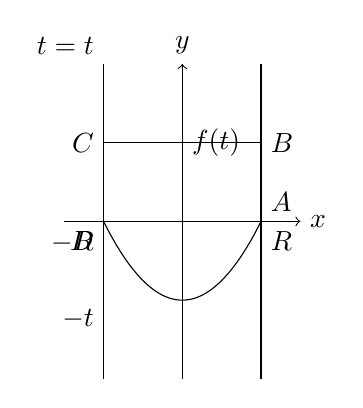
\begin{tikzpicture}
% Right diagram
\draw[->] (-1.5, 0) -- (1.5, 0) node[right] {$x$};
\draw[->] (0, -2) -- (0, 2) node[above] {$y$};
\draw (-1, -2) -- (-1, 2) node[above left] {$t=t$};
\draw (1, -2) -- (1, 2);
\node at (-1, 0) [below left] {$-R$};
\node at (1, 0) [below right] {$R$};
\draw (-1, 0) rectangle (1, 1);
\node at (0, 1) [right] {$f(t)$};
\draw[domain=-1:1, smooth, variable=\x] plot ({\x}, {\x*\x - 1});
\node at (-1, -1) [below left] {$-t$};
\node at (1, 1) [right] {$B$};
\node at (1, 0) [above right] {$A$};
\node at (-1, 0) [below left] {$D$};
\node at (-1, 1) [left] {$C$};
\end{tikzpicture}
\end{center}

\end{document}
